\documentclass{beamer}
% \usepackage[utf8]{inputenc}
\usepackage[T1]{fontenc}
\usepackage[upright]{fourier}
\usepackage[dvipsnames]{xcolor}
\usepackage{graphicx, float}
\graphicspath{{res/}}
\usepackage{tkz-kiviat,numprint}
\usepackage{amsfonts,amsmath,oldgerm}
\usetikzlibrary{arrows}
\thispagestyle{empty}
\usetheme{sintef}

\usefonttheme[onlymath]{serif}
\newcommand{\hrefcol}[2]{\textcolor{cyan}{\href{#1}{#2}}}
\newcommand{\testcolor}[1]{\colorbox{#1}{\textcolor{#1}{test}}~\texttt{#1}}

\titlebackground*{res/background}

\title{Social Engineering}
\subtitle{Bachelor Seminar - Billion Dollar Heist}
\author{Silas A. Kraume}
\date{}

\begin{document}
\maketitle

\section{Social Engineering}

\begin{frame}[fragile]{Was ist Social Engineering?}
    \begin{block}{Definition (grob)}
        \begin{verbatim}
"... eine zwischenmenschliche Beeinflussung durch diverse psycho-
logische Tricks zwecksgemäß konkrete Verhaltensmuster hervorzurufen"
        \end{verbatim}
    \end{block}
\end{frame}

\begin{frame}[fragile]{Was ist Social Engineering?}
    \begin{block}{Definition (geläufig)}
        \begin{verbatim}
"Social Engineering ist eine zwischenmenschliche Manipulation, bei der 
ein Unbefugter unter Vortäuschung falscher Tatsachen versucht,
unberechtigten Zugang zu Informationen oder IT-Systemen zu erlangen."
        \end{verbatim}
    \end{block}
    \begin{center}
        \Tiny{BKA, Social engineering / ceo-fraud, Oktober, 2017}
    \end{center}
    \nocite{bka}
\end{frame}

\begin{frame}{Methodik}
    \begin{figure}[!htp]
        \centering
        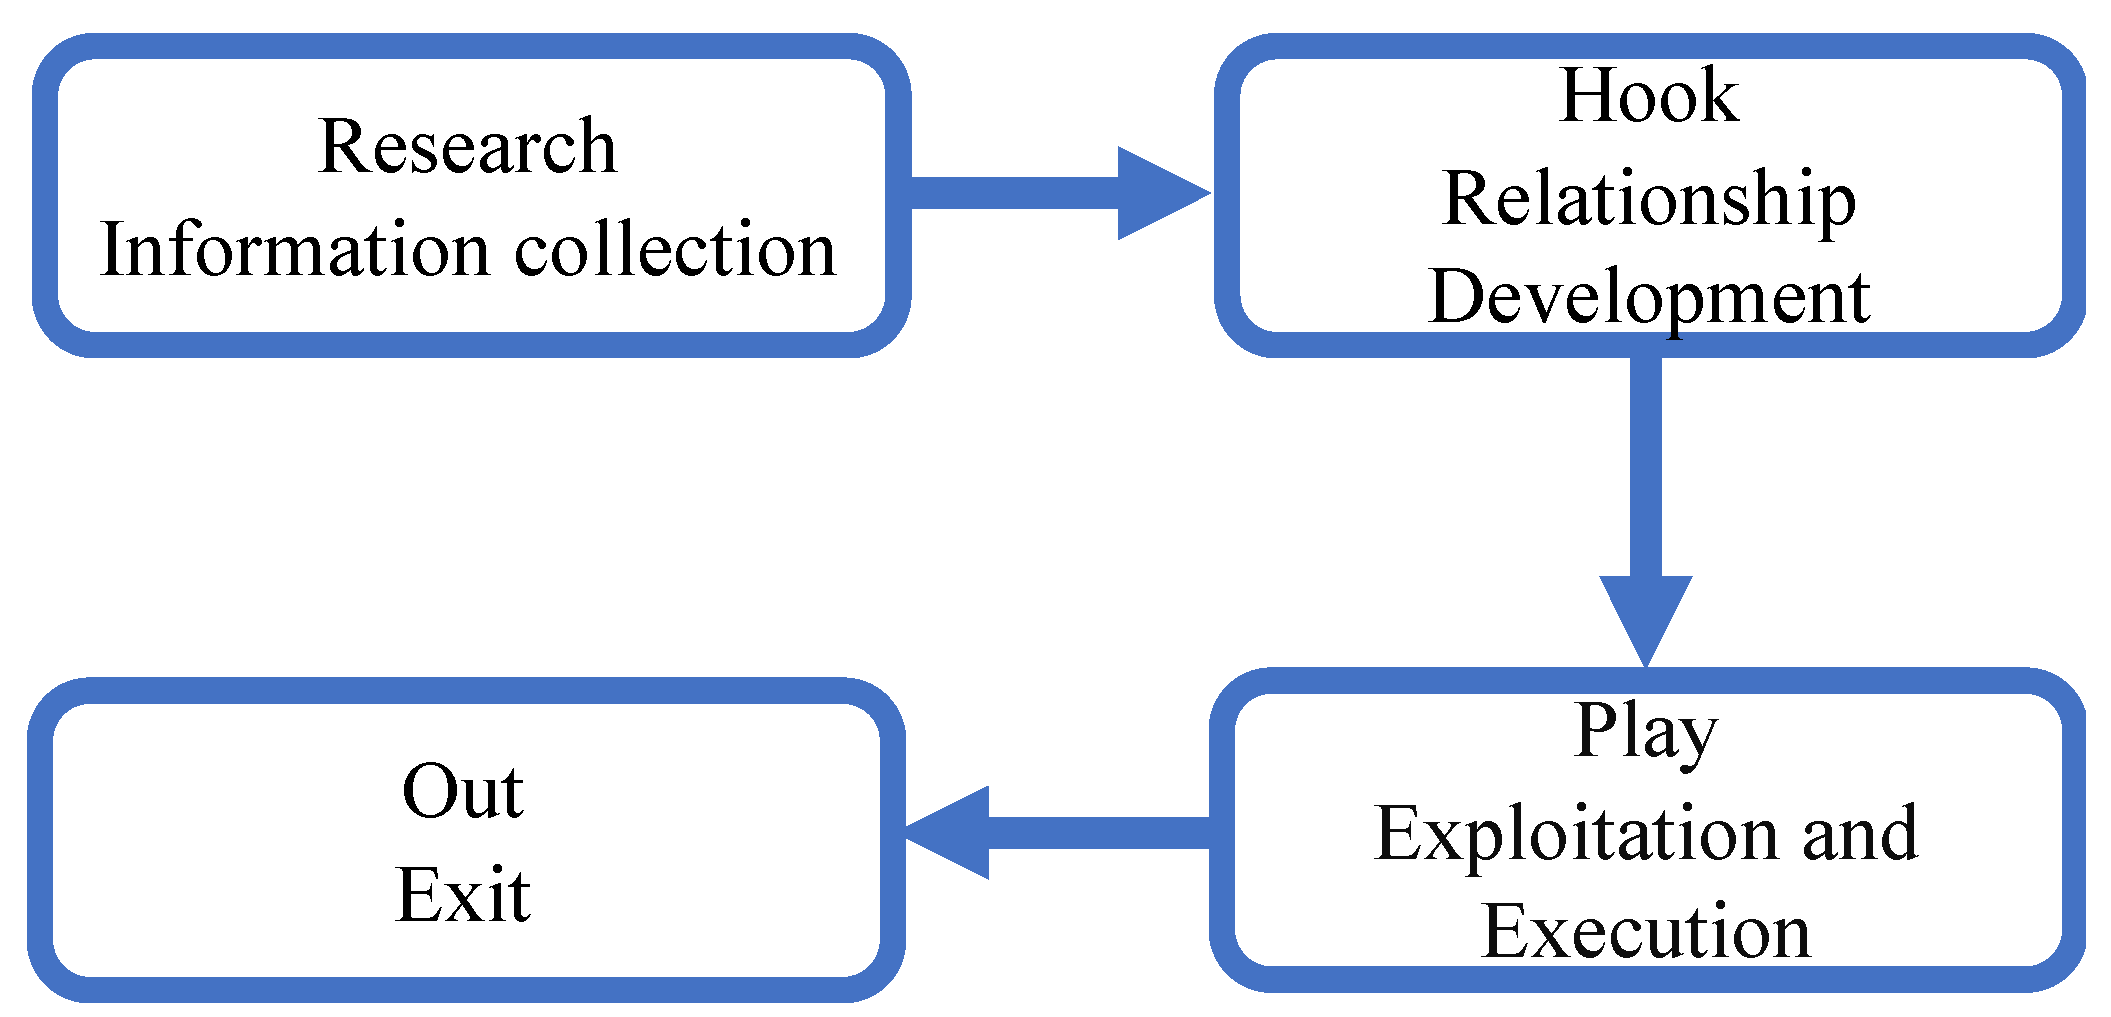
\includegraphics[scale=.15]{Methodik}
    \end{figure}
    \begin{center}
        \Tiny{Salahdine, F.; Kaabouch, N. Social Engineering Attacks: A Survey. Future Internet 2019, 11, 89. https://doi.org/10.3390/fi11040089}
    \end{center}
    \nocite{methodik}
\end{frame}

\begin{frame}{Klassifikation}
    \begin{figure}[!htp]
        \centering
        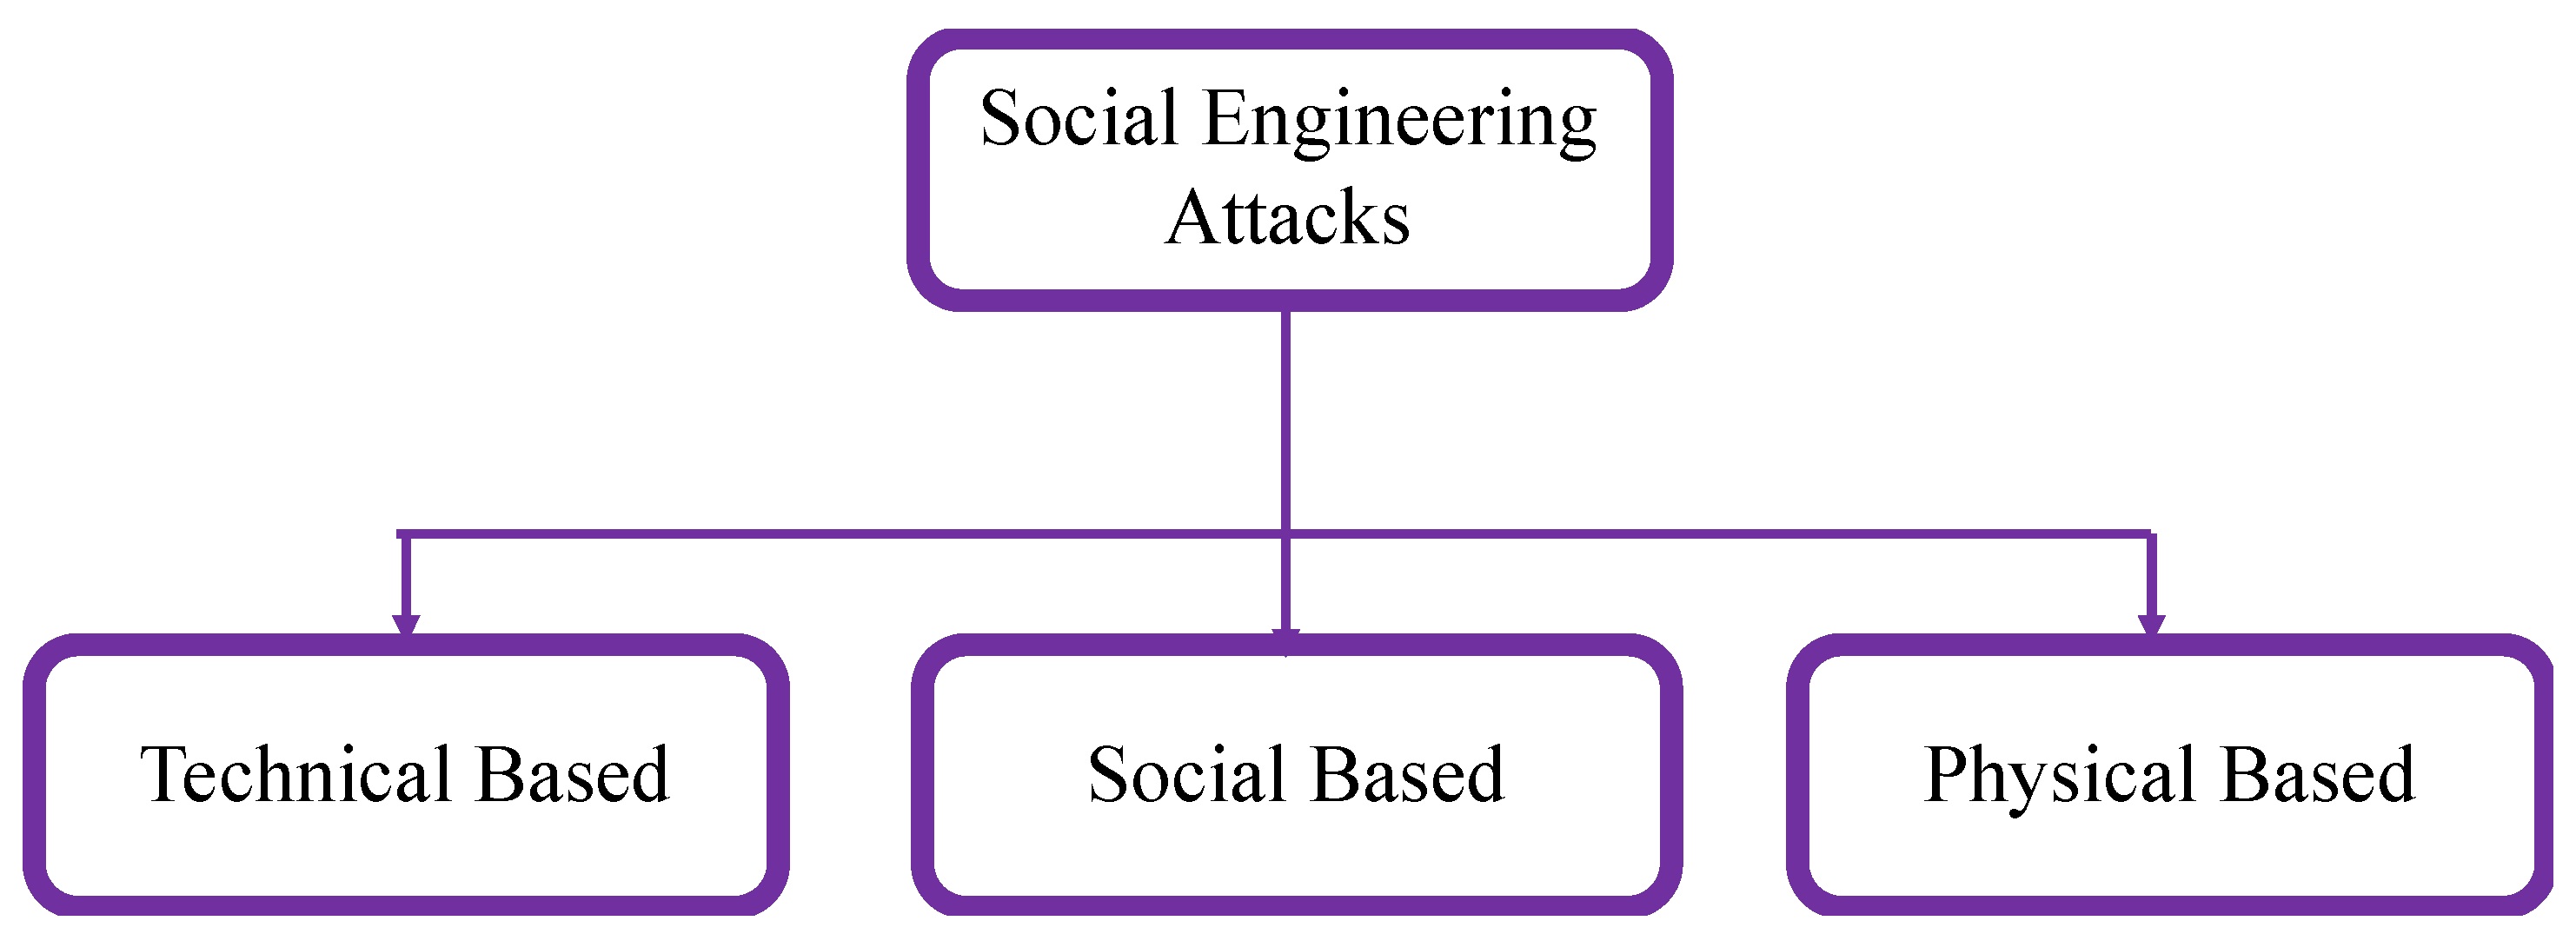
\includegraphics[scale=.12]{Klassifikation.png}
    \end{figure}
    \begin{center}
        \Tiny{Salahdine, F.; Kaabouch, N. Social Engineering Attacks: A Survey. Future Internet 2019, 11, 89. https://doi.org/10.3390/fi11040089}
    \end{center}
    \nocite{survey}
\end{frame}

\begin{frame}{Angriffsvektoren}
    \Large{
        \begin{itemize}
            \item Pretexting
            \item Phishing
            \item Baiting
            \item Tailgaiting
            \item Quid Pro Quo
            \item Reverse Social Engineering
            \item Deepfake
            \item ...
        \end{itemize}
    }
\end{frame}

\section{Gegenmaßnahmen}

\begin{frame}{Erkennung \& Vorbeugung}
    \Large{
        \begin{itemize}
            \item Legitimät prüfen
            \item verantwortungsvoller Umgang mit dem Internet
            \item Identifizierungs- und Authentifizierungsprozesse
            (grundsätzliche Sicherheitsmaßnahmen)
            \item Pen-Tests
            \item Bewusstsein schaffen
        \end{itemize}
    }
\end{frame}

% \begin{frame}{Juristik}
%     \begin{center}
%         \Large{Social Engineering ist allenfalls eine Täuschung!}
%     \end{center}
% \end{frame}

% \section{Auswirkungen}

% TODO: 

\section{Psychologie}

\begin{frame}{Persönlichkeitspsychologie \space\space\space\small{OCEAN/Big Five-Modell}}
    \begin{center}
        \begin{tikzpicture}
            \tkzKiviatDiagram[scale=1.5,label distance=1.1cm,
                radial  = 1,
                gap     = 0.3,
                lattice = 5, label space = 0.7]{\newline\newline Offenheit,Gewissenhaftigkeit,Extraversion,Verträglichkeit,Neurotizismus}
            \tkzKiviatLine[thick,color=blue,mark=none,
                fill=blue!20,opacity=.5](4.25,4.65,2.8,4.35,2.8) % 85, 93, 56, 87, 56
            \tkzKiviatGrad[unity=20](1)
        \end{tikzpicture}
    \end{center}
\end{frame}

\begin{frame}{Anfälligkeit für Social Engineering}
    \begin{figure}[!htp]
        \centering
        \includegraphics[scale=.45]{Anfälligkeit}
    \end{figure}
    \begin{center}
        \Tiny{S. Uebelacker and S. Quiel, "The Social Engineering Personality Framework," 2014 Workshop on Socio-Technical Aspects in Security and Trust, Vienna, Austria, 2014, pp. 24-30, doi: 10.1109/STAST.2014.12.}
    \end{center}
    \nocite{ffm}
\end{frame}

\section{Zusammenfassung}

\begin{frame}
    \frametitle{Fazit!}
    \Large{
        \begin{itemize}
            \item Social Engineering ist im ständigen Wandel
            % \item Es herrscht eine nie zuvor gesehene Angriffsflut
            \item Jeder ist angreifbar
            \item Das Bewusstsein ist die beste Abwehr
        \end{itemize}
    }
\end{frame}

\begin{frame}
    \frametitle{Danke!}
    \begin{center}
        \LARGE{Vielen Dank für Eure Aufmerksamkeit!}
    \end{center}
\end{frame}

\section{Quellen}

\begin{frame}[allowframebreaks]
    \frametitle{Quellenverzeichnis}
    \bibliographystyle{amsalpha}
    \bibliography{references}
\end{frame}

\end{document}
